\documentclass[12pt]{report}
\usepackage[french]{babel}

\usepackage[T1]{fontenc}
\usepackage{amstext}
\usepackage{amssymb}
\usepackage{amsmath}
\usepackage{graphicx}
\usepackage[utf8]{inputenc}
\usepackage{babel}
\usepackage{hyperref}
\usepackage{float}
\usepackage{subcaption}

\usepackage[a4paper,top=3cm,bottom=2cm,left=2cm,right=2cm,marginparwidth=1.75cm]{geometry}  % pour configurer les marges
%%%%%%%%%% Start TeXmacs macros
\newcommand{\tmmathbf}[1]{\ensuremath{\boldsymbol{#1}}}
\newcommand{\tmop}[1]{\ensuremath{\operatorname{#1}}}
%%%%%%%%%% End TeXmacs macros

\makeatletter

\providecommand{\tabularnewline}{\\}

\makeatother

\begin{document}


\begin{titlepage}

\newcommand{\HRule}{\rule{\linewidth}{0.5mm}} % Defines a new command for the horizontal lines, change thickness here

\center % Center everything on the page
 
%----------------------------------------------------------------------------------------
%   HEADING SECTIONS
%----------------------------------------------------------------------------------------

\vspace{3cm}
\textsc{\LARGE Kévin REN,  Théo MASSA \\[0.5cm] Guillaume GARDE, Hugo HOFMANN } \\ [1.5cm]
\textsc{\Large UV 6.1 -- Projet au lac de Guerlédan}\\[1.5cm]

%----------------------------------------------------------------------------------------
%   TITLE SECTION
%----------------------------------------------------------------------------------------
\HRule \\[0.4cm]
{ \huge \bfseries \textsc{Docking\\[0.3cm]}}
\HRule \\[.5cm]

%----------------------------------------------------------------------------------------
%   DATE SECTION
%----------------------------------------------------------------------------------------

\vspace{1cm}
{\huge \today}\\[1cm] % Date, change the \today to a set date if you want to be precise

%----------------------------------------------------------------------------------------
%   LOGO SECTION
%----------------------------------------------------------------------------------------
% \raggedright
\vspace{2cm}
% 
\includegraphics[width = 5.5cm]{logo.pdf}\\[1cm] % Include a department/university logo - this will require the graphicx package

\includegraphics[width=6cm]{imgs/logo_ensta.jpg}

\includegraphics[width=6cm]{imgs/logo-lab-sticc2.png}

\includegraphics[width=6cm]{imgs/logo_ubs_transparent.png} 
%----------------------------------------------------------------------------------------

\vfill % Fill the rest of the page with whitespace

\end{titlepage}

\tableofcontents

\chapter{Introduction}

\section{Présentation du sujet}

Que ce soit dans le monde de la recherche ou dans les différents domaines dans lesquels sont utilisés les drones et tout particulièrement les AUV ou UAV, l'une des grandes difficultés rencontrées est très certainement celle du docking. En effet, bien qu'il faille tôt ou tard récupérer le drone à la fin de sa mission ou en cas de problème, cela peut se révéler dans le meilleur des cas fastidieux (dans le cas ou la manoeuvre est manuelle par exemple) et dans le pire des cas difficile voire dangereux pour le drone (dans le cas d'une mer agitée par exemple). Dans le cas d'une mission autonome loin du bateau, on comprend qu'il peut être très intéressant de développer une solution de docking autonome, permettant au drone de revenir vers sa base tout seul et avec précision. L'objectif de ce projet Guerlédan sera donc de développer cette solution en s'intéressant au cas d'un AUV sur le lac. Les objectifs seront les suivants:

\begin{enumerate}
    \item Le drone doit être capable de planifier et réaliser son retour vers le dock
    \item Le dock doit pouvoir communiquer sa position et son attitude en temps réel et potentiellement à longue distance pour que le drone puisse effectuer son retour peu importe la position (parfois changeante) du dock
    \item Le docking doit se faire avec une précision suffisante (à la dizaine de centimètres voire mieux) pour que le drone puisse correctement entrer dans la structure
\end{enumerate}

\section{Matériel à disposition}
La majorité du matériel nécessaire nous a directement été fournie. En voici une liste (non exhaustive).
\subsection{Dock}
Pour ce qui est du dock, nous avions déjà les éléments nécessaires :

\begin{itemize}
    \item Un récepteur GNSS \textit{Ublox} monté sur une carte \textit{ArduSimple}
    \item Une antenne radio \textit{Xbee} pour recevoir les corrections RTK
    \item Une IMU \textit{SBG Ellipse A}
    \item \textit{NVIDIA Jetson Nano avec ROS}
\end{itemize}

Quant à la structure en elle-même du dock, nos encadrants ont fourni pour la deuxième semaine d'expérimentations un dock \ref{fig:dock} permettant d'accueillir le drone.
Puisque la mission nécessite que le dock communique avec le drone, et ce à longue distance, nous avons également reçu deux modems \textit{Simpulse SL200}\ref{fig:simpulse} qu'il a fallu configurer.

\begin{figure}[H]
    \begin{subfigure}{0.45\textwidth}
        \centering
        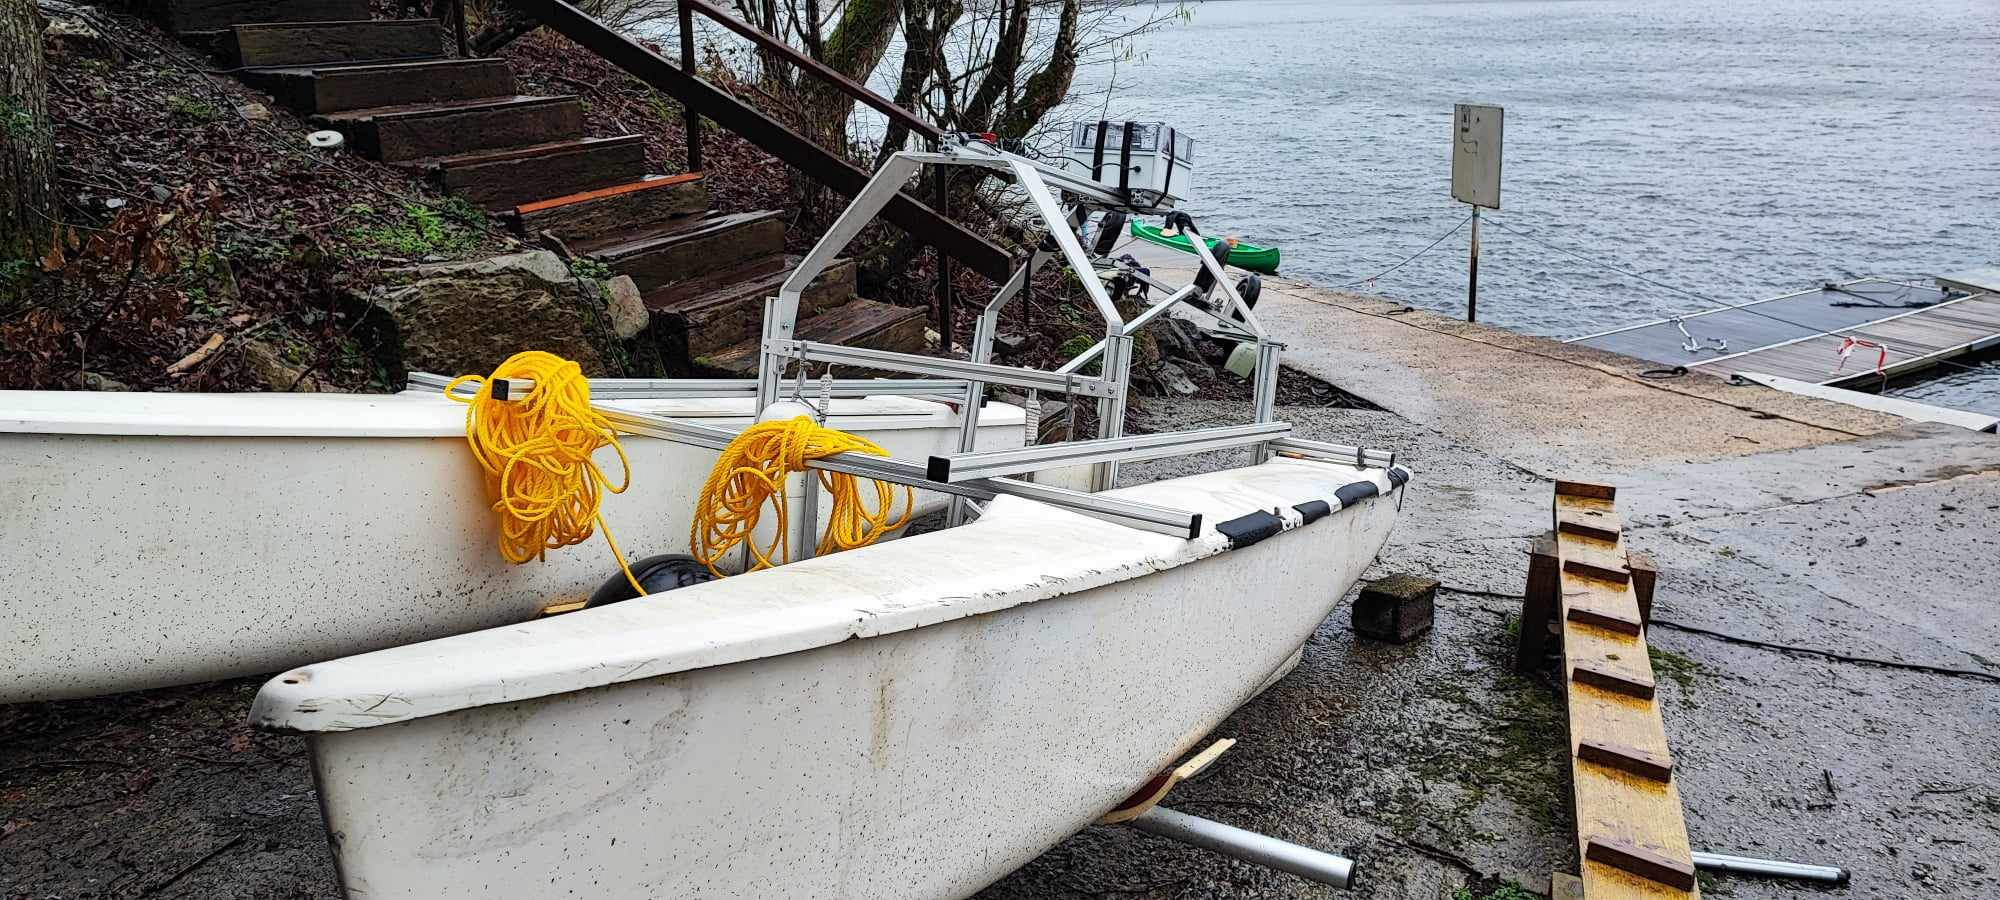
\includegraphics[width=0.8\textwidth]{imgs/dock.jpg}
        \caption{Le dock}
        \label{fig:dock}
    \end{subfigure}
    \begin{subfigure}{0.4\textwidth}
        \centering
        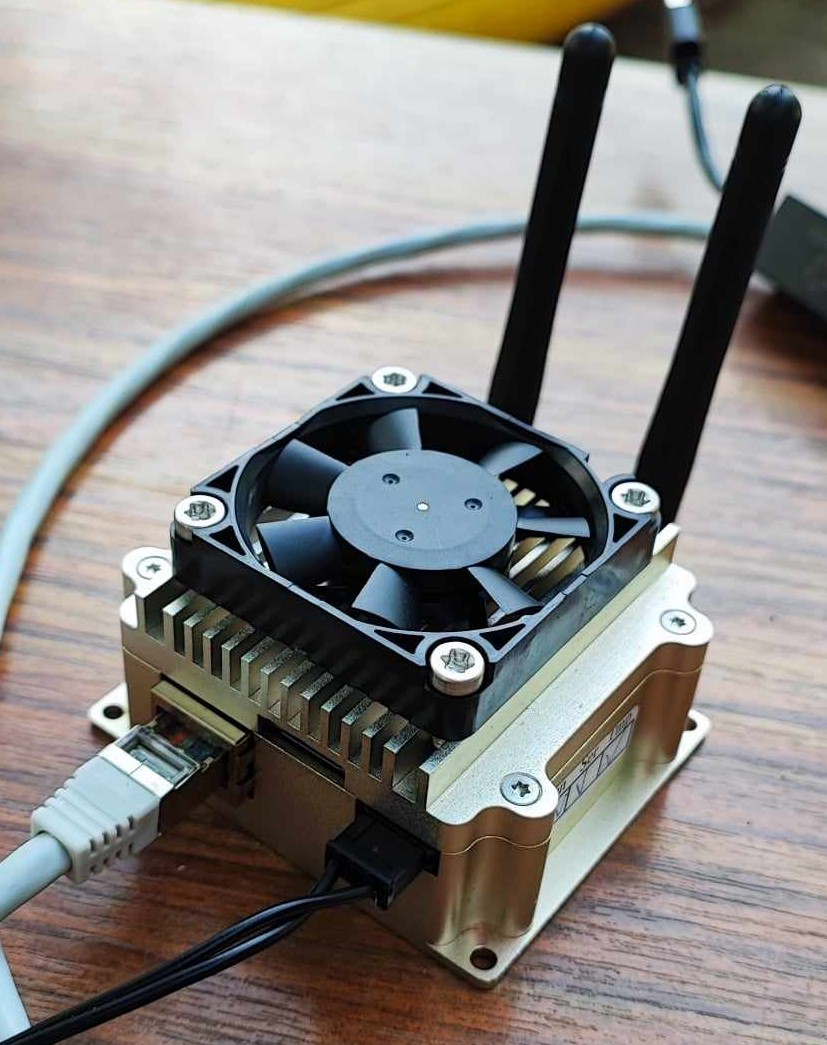
\includegraphics[width=0.4\textwidth]{imgs/simpulse.jpg}
        \caption{Modem Simpulse}
        \label{fig:simpulse}
    \end{subfigure}
    \caption{Matériel fourni}
\end{figure}

\subsection{Drone AUV}
Pour ce qui est de l'AUV, nous avons pu travailler (seulement le temps des deux semaines sur le lac) avec le \textit{M1800} d'\textit{IMSolutions}.
\begin{figure}[H]
    \centering
    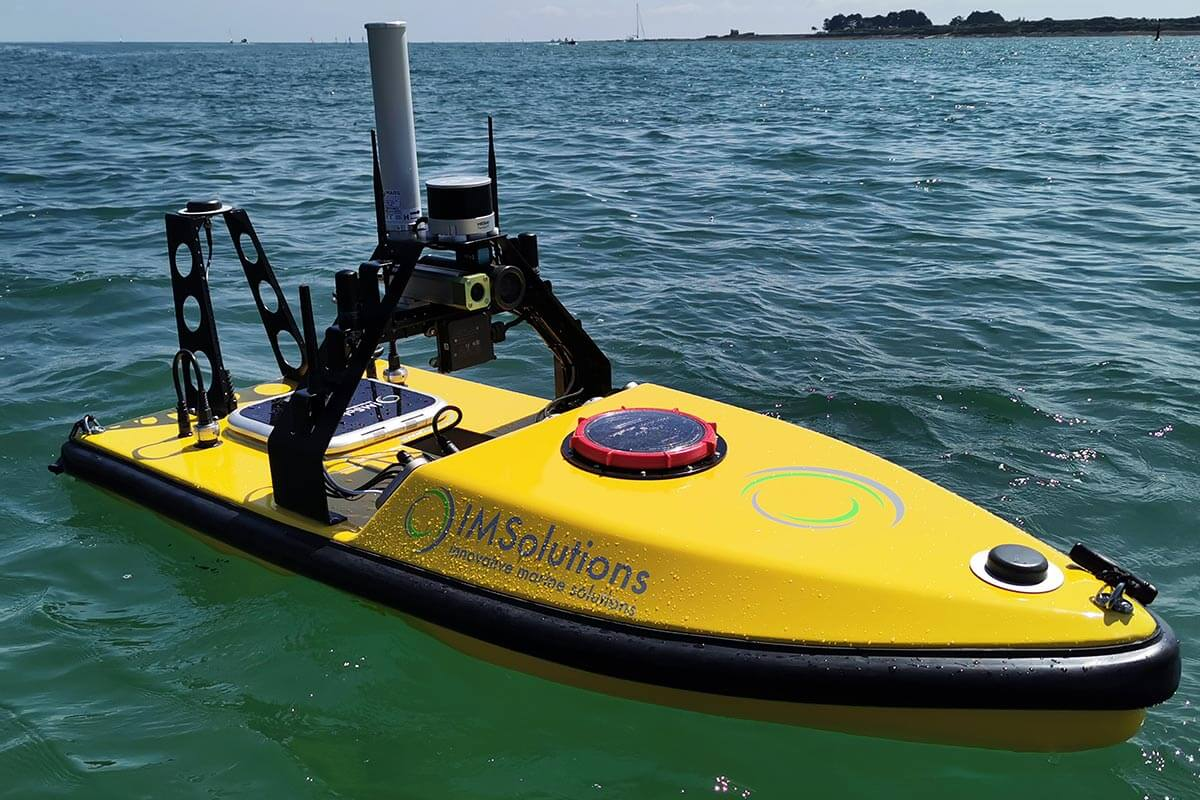
\includegraphics[width=0.5\textwidth]{imgs/monodrone-1800-chenal.jpg}
    \caption{L'AUV en question, sans les capteurs supplémentaires}
\end{figure}
Le drone embarque déjà tous les capteurs nécessaires à la mission comme elle a été envisagée :

\begin{itemize}
    \item Récepteur GNSS RTK
    \item IMU \textit{SBG Ellipse D}
\end{itemize}

Sur le modèle exact qui nous a été fourni, de nombreux autres capteurs tels que des caméras et un LIDAR ont été montés; s'ils n'ont pas été utilisés pendant la mission (dont le plus important était surtout dans un premier temps l'approche du drone vers le dock), ils pourraient en revanche se révéler utiles dans un second temps pour de prochaines expérimentations sur le projet.
\subsection{Rover}

Puisque le drone n'était disponible que peu de temps et uniquement lors des semaines à Guerlédan, nous avions besoin d'un remplacement pour pouvoir continuer à travailler et tester nos algorithmes à l'ENSTA. C'est pour cela que nous avons pu travailler avec l'\textit{AION R1}\ref{fig:rover}, un rover à la structure software équivalente à celle du drone (tournant sous \textit{ROS}, et gérant les commandes moteurs via une carte \textit{Pixhawk}). On peut ainsi commander le rover exactement de la même manière que l'AUV, c'est-à-dire dans notre cas lui envoyer des commandes en vitesses linéaire et angulaire.

\begin{figure}[H]
    \centering
    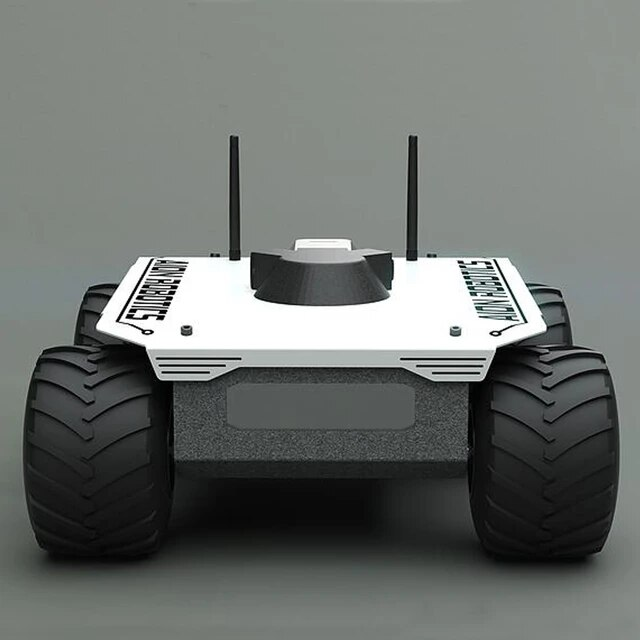
\includegraphics[width=0.4\textwidth]{imgs/rover.jpg}
    \caption{l'\textit{AION Robotics R1}}
    \label{fig:rover}
\end{figure}

\chapter{Conception du dock}
\section{Mise en place d'une base RTK}
Le positionnement GPS acquis par les capteurs à disposition confère une précision métrique, les signaux GPS étant perturbés par l'atmosphère. Or, il faut de meilleures performances pour espérer docker le drône dans un environnement confiné et restreint. 
L'idée était donc de mettre en place un système de positionnement plus précis (centimétrique dans l'idéal) en  utilisant le dispositif du \textit{Real Time Kinematic} (RTK).
Pour cela, il faut installer une base GPS fixe de position connue précisément. Elle servira de médiateur en diffusant des corrections de positionnement aux systèmes GPS connectés.
L'installation est donc en deux parties, la première, à terre, l'autre, directement sur le dock.
\subsection{Capteurs à disposition}
L'acquisition de signaux GPS se fait grâce à deux modules \textit{ArduSimple} équipés de processeurs \textit{u-blox ZED-F9P}. 
% //TODO : images ?
Les deux modules communiquent grâce à leur antenne radio \textit{Xbee S2C 2,4 GHz}. La base dispose d'une antenne GPS qui permet une meilleure acquisition des signaux. 
Il est possible d'utiliser une \textit{Raspberry} pour configurer la base GPS en lui conférant une interface graphique. Un guide de configuration des capteurs est disponible en annexe.

\subsection{Installation de la base}
L'installation de la base peut se faire de deux manières différentes. 
\begin{enumerate}
    \item En utilisant uniquement le module \textit{u-blox}. Il s'agit de la méthode la plus simple. Si la position précise de la base est connue, on configure le module en \textit{Fixed Mode} et les corrections seront directement disponibles. 
    Sinon on le configure en mode \textit{Survey-In} ce qui va lancer l'acquisition de trames GPS provenants de satellites jusqu'à ce que la position soit connue avec une précision suffisante. Cela peut prendre une dizaine d'heures pour une précision centimétrique. La configuration du module se fait avec le logiciel \textit{XCTU}(sous Windows). Dans tous les cas, il faut que la base soit alimentée en permanence pour ne pas perdre la position acquise et que l'antenne soit bien dégagée pour une meilleure réception des signaux.
    \item En utilisant le module \textit{u-blox} et une \textit{Raspberry}. Cette solution est issue de la documentation fournie par \textit{Centipède} pour la mise en place d'une base RTK déclarée sur leur réseau. 
    Dans ce cas, aucun \textit{TimeMode} n'est spécifié pour le module GPS. La \textit{Raspberry} est flashée et configurée pour enregistrer les trames GPS reçues par le \textit{u-blox} puis faire une sauvegarde par jour (vers 4h du matin). 
    L'idée est ensuite de récupérer une sauvegarde de 24 heures, de l'envoyer à \textit{IGN} qui fournit un service de triangulation. \textit{IGN} renvoie ensuite la position précise calculée à partir des données. 
    A partir d'ici, il n'est plus nécessaire de suivre les instructions de \textit{Centipède}\footnote{Le but n'est pas de déclarer la base sur leur réseau.}. Il faut en revanche passer le module \textit{u-blox} en mode \textit{Fixed Mode} et renseigner la position déterminée précédemment. 
    Avec la \textit{Raspberry}, on peut accéder aux données directement en se connectant en \textit{ssh} ou alors en se connectant à l'interface web graphique de la carte.
\end{enumerate}

Une fois l'installation terminée, la base RTK diffuse ses corrections de positionnement à l'aide de l'antenne radio \textit{Xbee}. Le statut de la base est indiqué par les LEDs de la carte \textit{ArduSimple}.
\begin{itemize}
    \item GPS FIX : \textbf{OFF} lorsqu'il n'y a pas de fix, \textbf{une impulsion par seconde} lorsque la position est valide.
    \item NO RTK : \textbf{OFF} lorsque RTK fixe, \textbf{clignotant} lors de la réception de données RTCM, \textbf{ON} lorsqu'aucune correction n'a lieu. 
    \item GPS$\rightarrow$ XBEE : \textbf{clignotant} lorsque le module GPS envoie des données à l'antenne radio.
\end{itemize}
\subsection{Configuration du dock}
La configuration du dock est plus courte. Il suffit d'alimenter le module \textit{u-blox} et de le connecter à une antenne. La configuration précise est donnée en annexe. Une fois alimenté, le module va acquérir les signaux satellites et les corrections RTK envoyées par la base. 
Si jamais aucune correction n'est reçue, le \textit{u-blox} va fournir une position GPS classique. Les LEDs fournissent les indications utiles : 
\begin{itemize}
    \item GPS FIX : \textbf{OFF} lorsqu'il n'y a pas de fix, \textbf{une impulsion par seconde} lorsque la position est valide.
    \item NO RTK : \textbf{OFF} lorsque RTK fixe, \textbf{clignotant} lors de la réception de données RTCM, \textbf{ON} lorsqu'aucune correction n'a lieu. 
    \item XBEE $\rightarrow$ GPS : \textbf{clignotant} lorsque le module GPS reçoit des données de l'antenne radio.
\end{itemize}

\subsection{Un mot sur les antennes}
Les antennes de communication des deux modules GPS sont des \textit{XBEE S2C 2,4 GHz}. Elles doivent être correctement paramétrées pour pouvoir échanger. 
Les spécifications sont données en annexe.

\section{Mise en place du dock}

L'ensemble de l'électronique embarquée du dock tient dans une boîte étanche qui laisse passer le câble de l'IMU. En effet, pour pouvoir s'assurer du bon fonctionnement cette dernière sa calibration a été réalisée grâce au logiciel \textit{SBG Center} tout d'abord en la plaçant à l'intérieur de la boîte avec le reste de l'électronique. Or en observant les valeurs données et en essayant la calibration il apparaissait que les appareils aux alentours produisaient des perturbations magnétiques bien trop importantes pour que le cap mesuré soit cohérent. C'est pour cela qu'il a été décidé de plutôt placer l'IMU en dehors de la boîte pour pouvoir qu'elle fonctionne correctement (cf ~\ref{fig:IMU_exterieur}).

\begin{figure}[H]
    % \centering
    \begin{subfigure}{0.54\textwidth}
        \centering
        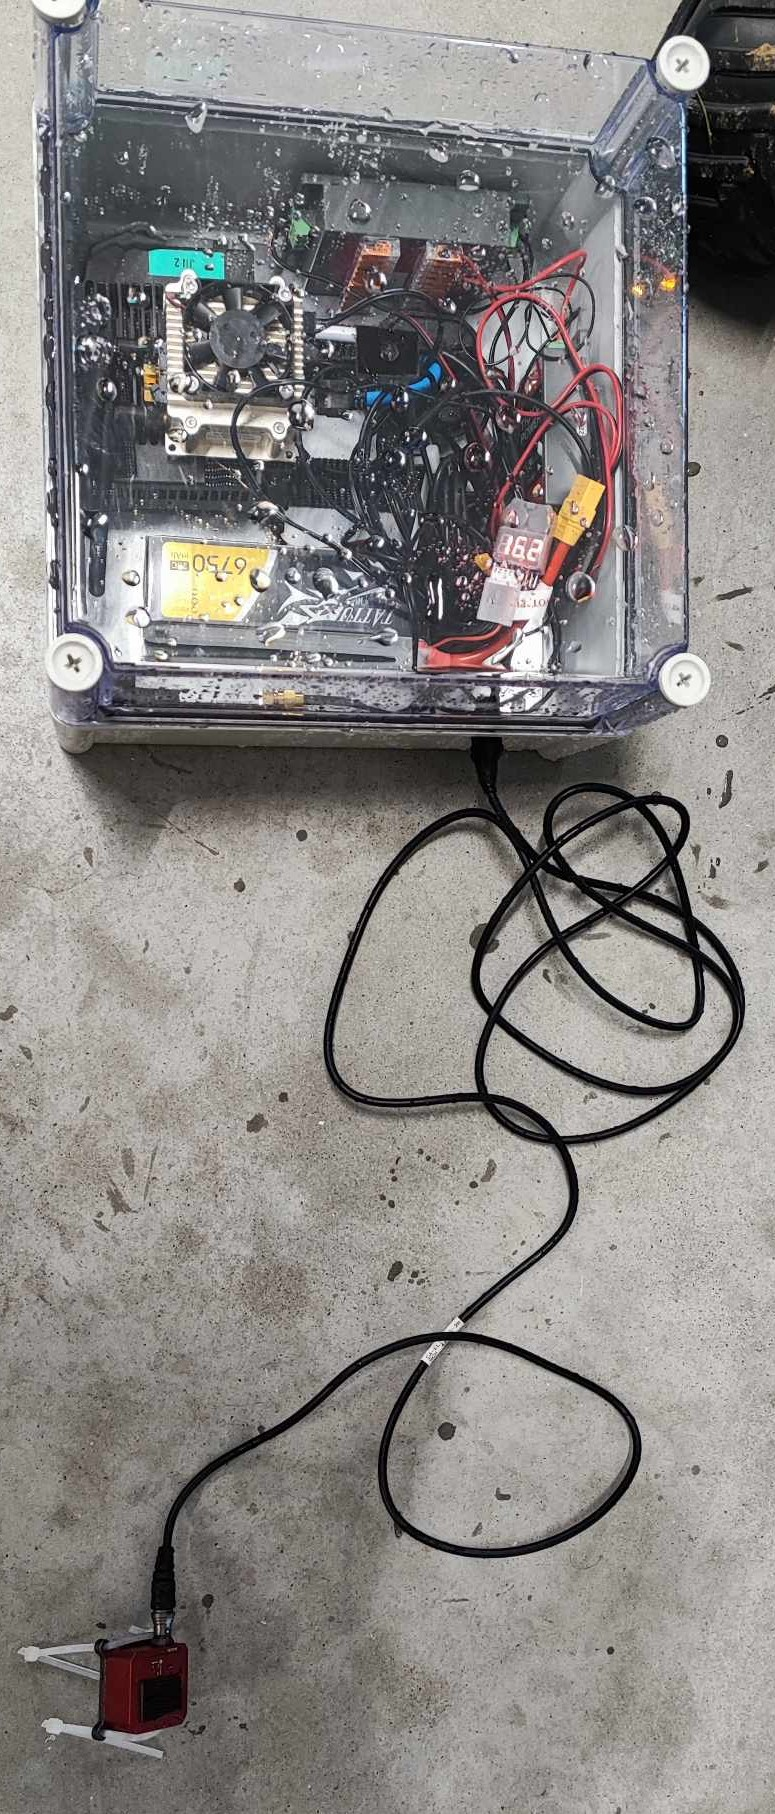
\includegraphics[height=\textwidth,angle=90]{imgs/dock_box_outside.jpg}
        \caption{Le bloc entier à monter sur la structure (droite : IMU)}
        \label{fig:IMU_exterieur}
    \end{subfigure}
    \begin{subfigure}{0.45\textwidth}
        \centering
        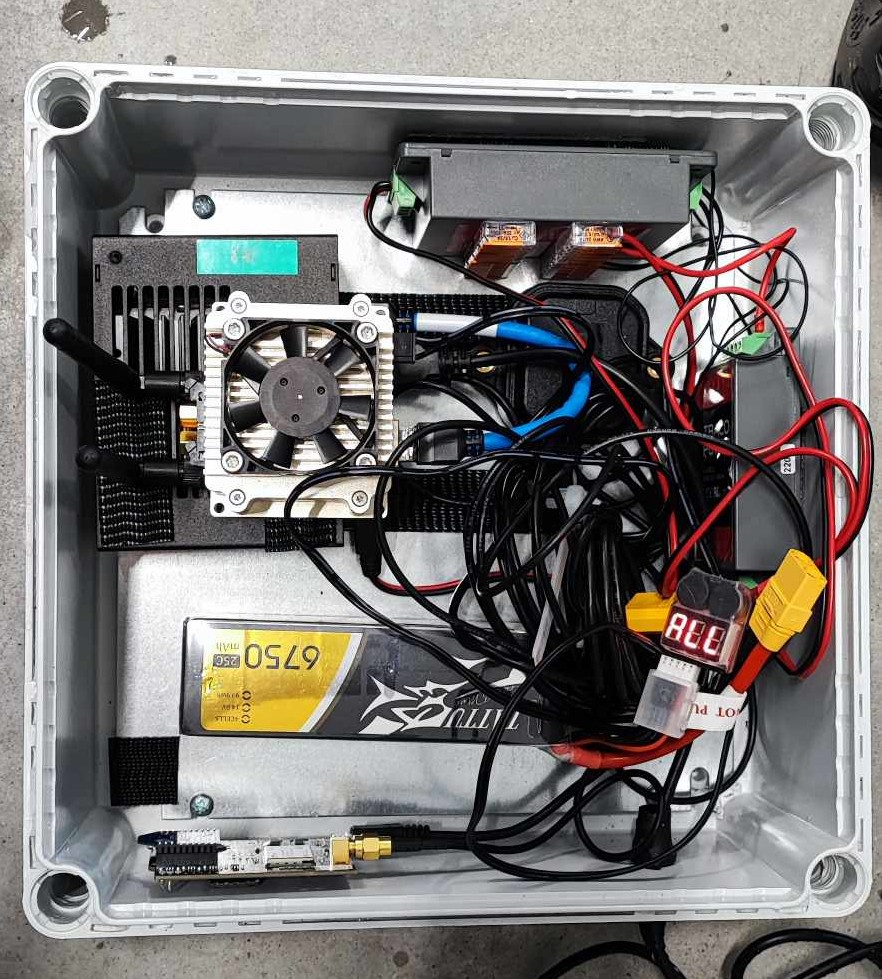
\includegraphics[width=0.95\textwidth]{imgs/dock_box_inside.jpg}
        \caption{Intérieur du dock avec toute l'électronique}
    \end{subfigure}
    \caption{Mise en place du dock}
\end{figure}

\section{Communication avec le reste du système}

Pour rappel, le dock doit pouvoir envoyer sa position et son attitude au drone pour que ce dernier puisse planifier son retour, et ce potentiellement à longue distance.  C'est pour cela que dans le cadre de ce projet nous utilisons des modems \textit{Simpulse}. S'il est possible de communiquer entre noeuds ROS, ce n'est pas l'approche qui sera finalement utilisée : outre les difficultés dues à ROS (qui n'existent pas en ROS2), on préfèrera aussi un protocole plus simple et plus universel pour que la communication s'adapte facilement sur d'autres OS ou appareils (par exemple, si le dock et le drone ont des versions différentes de ROS, la communication directe n'est pas possible). La communication se fait donc en UDP (quoi qu'on aurait pu choisir le TCP qui permet une garantie sur la bonne réception, cela n'était pas absolument nécessaire); on veut donc envoyer des trames à intervalle régulier contenant les informations nécessaires que sont la position GPS et l'attitude du dock. On peut donc définir un format simple permettant de véhiculer ces informations :

\verb|${latitude},{longitude};{roll},{pitch},{yaw}|

On précise que l'utilisation des angles d'Euler, faciles à interpréter lors du débuggage, est justifiée par le fait que dans notre cas on ne risque pas le \textit{Gimbal lock} vus les angles relativement faibles sur le pitch et le roll.

La communication se fait donc assez facilement de cette manière, après avoir bien configuré les addresses du dock et du drone.

\begin{figure}[H]
    \centering
    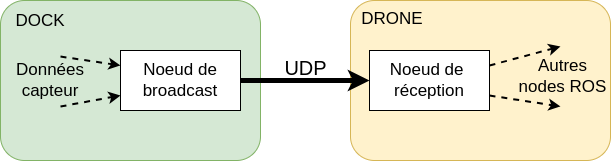
\includegraphics[width=0.6\textwidth]{imgs/UDP_connexion.png}
    \caption{La communication dock $\rightarrow$ drone}
\end{figure}

La trame est ensuite interprétée et convertie en messages ROS publiés sur des topics et utilisés par le reste du système.


\chapter{Stratégie d'approche de docking}

\section{Filtre de Kalman}

Le modèle cinématique choisi pour le robot est le suivant :
\begin{eqnarray}
     \mathbf{\dot{x}} & = & B \mathbf{u} \nonumber\\
     \label{eq:cinematic} \left( \begin{array}{c}
       \dot{x}\\
       \dot{y}\\
       \dot{z}\\
       \dot{\psi}
     \end{array} \right) & = & \left( \begin{array}{cc}
       \cos (\varphi) \cos (\psi) & 0\\
       \cos (\varphi) \sin (\psi) & 0\\
       - \sin (\varphi) & 0\\
       0 & 1
     \end{array} \right) \left( \begin{array}{c}
       v\\
       \omega
     \end{array} \right) 
   \end{eqnarray}
où $(x, y, z)$ représente les coordonnées du robot dans le repère ENU, $\varphi$ représente l'assiette et $\psi$ le cap.

Ce modèle est issu du modèle de Dubins mais où contrairement à ce dernier, on suppose que le véhicule est commandé en vitesse. Cette décision a été prise parce que le rover et le bateau sont commandés à l'aide d'un message de type cmd\_vel, qui spécifie à la fois la vitesse linéaire et la vitesse angulaire.

Le modèle cinématique étant choisi, le modèle d'observation peut être défini. À l'heure actuelle, seules les données de position GPS $(x, y)$ et de cap $\psi$ sont intégrées par le filtre.
\begin{eqnarray}
  \mathbf{y} & = & C \mathbf{x} \nonumber\\
  \label{eq:obs} \left( \begin{array}{c}
    x\\
    y\\
    \psi
  \end{array} \right) & = & \left( \begin{array}{cccc}
    1 & 0 & 0 & 0\\
    0 & 1 & 0 & 0\\
    0 & 0 & 0 & 1
  \end{array} \right) \left( \begin{array}{c}
    x\\
    y\\
    z\\
    \psi
  \end{array} \right) 
\end{eqnarray}
Les matrices de covariance ont été déterminées à posteriori et sont évidemment à ajuster plus tard. Notons $Q$ la matrice de covariance du bruit d'évolution et $R$ la matrice de covariance du bruit de mesure, nous avons pris :
\[ \left\{ \begin{array}{c}
     Q = \left( \begin{array}{ccc}
       .5 & 0 & 0\\
       0 & .5 & 0\\
       0 & 0 & .5
     \end{array} \right)\\
     R = \left( \begin{array}{ccc}
       1 & 0 & 0\\
       0 & 1 & 0\\
       0 & 0 & .17
     \end{array} \right)
   \end{array} \right. \]
Le filtre de Kalman s'appliquant sur un système discret, il faut discrétiser \eqref{eq:cinematic}. Ainsi au premier ordre nous avons
\begin{eqnarray}
  \mathbf{x} (t + dt) & = & \mathbf{x} (t) + \int_t^{t + dt}
  \dot{\mathbf{x}} (\tau) d \tau \nonumber\\
  & = & \mathbf{x} (t) + \int_t^{t + dt} B \mathbf{u} (\tau) d
  \tau \nonumber\\
  & = & \mathbf{x} (t) + dt B \mathbf{u} (t) \nonumber
\end{eqnarray}
La relation \eqref{eq:obs} peut quant à elle être directement utilisée. Il faut également discrétiser les matrices de covariances. On montre que
\[ \left\{ \begin{array}{c}
     \Gamma_{\alpha_k} = dt \Gamma_{\alpha}\\
     \Gamma_{\beta_k} = \frac{1}{dt} \Gamma_{\beta}
   \end{array} \right. \]

\section{Guidage par champ de potentiel artificiel}

Le guidage par champ de potentiel artificiel est un principe largement utilisé dans le domaine de la robotique mobile pour la navigation autonome des robots. L'idée fondamentale est de créer un champ de potentiel artificiel dans l'environnement dans lequel se déplace le robot, de telle sorte que le robot soit attiré vers sa destination et repoussé des obstacles.

Soit $\mathbf{v}$ le vecteur vitesse du robot et $M$ sa position. Formellement, le champ de potentiel peut être modélisé par une fonction $U : \mathbb{R}^2 \rightarrow \mathbb{R}$. Le robot devra ensuite être contrôlé de sorte que :
\[ \mathbf{v} (M) = - \vec{\nabla} U (M) \]

\subsection{Champ de potentiel retenu}

\subsubsection{Idée générale}

L'idée est d'adapter le champ de potentiel suivant la position $M$ du robot. Il y a deux cas possibles :
\begin{itemize}
  \item Le robot se trouve dans le demi-plan devant le dock (cas 1)
  
  \item Le robot se trouve dans le demi-plan derrière le dock (cas 2)
\end{itemize}
\begin{figure}[h]
  \centering
  \includegraphics[width=12.87cm,height=5.48cm]{imgs/RapportGuerlédan-image-1.png}
  \caption{La flèche indique la position et l'orientation du dock et le point représente la position du robot (a) À gauche le robot se trouve dans le demi-plan en face du robot (b) À droite le robot se trouve dans le demi-plan derrière le robot}
\end{figure}

Dans le premier cas le robot va aller sur la droite passant par le dock et dirigé dans le même sens que le dock. Dans le second cas le robot va d'abord aller dans le demi plan en face de robot en suivant un champ de vecteur uniforme tout en faisant attention à pas rentrer dans le dock - ce dernier devenant un point répulsif -. Puis en étant assez éloigné loin du demi plan en face du dock, le robot se retrouvera dans le premier cas et agira en conséquence.

\subsubsection{Mise en équation}

Soit $M$ la position du robot et $M'$ la position du dock. En s'inspirant des champs de potentiels physique comme le champ électrostatique, le champ de potentiel engendré par un point répulsif peut être défini ainsi :
\[ U_1 (M) = \frac{1}{\| \overrightarrow{M M'} \|^{\alpha}} \]
où $\alpha \in \mathbb{R}$ est un coefficient déterminant la répulsivité du point.

Le champ de potentiel d'une ligne attractive peut quant à lui être défini par :
\[ U_2 (M) = \overrightarrow{M' M}^T \cdot \vec{n} \cdot \vec{n}^T \overrightarrow{M' M} \]
Ce champ permet d'attirer le véhicule sur la ligne. Le véhicule arrive perpendiculairement à cette dernière et s'arrête ce qui signifie que le robot n'est pas bien orienté.

Enfin le champ de potentiel issu d'un champ de vecteur vitesse uniforme $\overrightarrow{v_d}$ peut être défini par :
\[ U_3 (M) = - \overrightarrow{v_d}^T \overrightarrow{OM} \]
Les champs de vitesses correspondant à chacun des champs de potentiels sont alors :
\[ \begin{array}{c}
     \begin{array}{c}
       \overrightarrow{v_1} = \frac{\overrightarrow{M' M}}{\| \overrightarrow{M M'} \|^{\alpha + 2}}
     \end{array}\\
     \overrightarrow{v_2} = - 2 \vec{n} \cdot \vec{n}^T \cdot \overrightarrow{M' M}\\
     \overrightarrow{v_3} = \overrightarrow{v_d}
   \end{array} \]


Dans le premier cas, il faut une ligne attractive pour positionner le robot sur la ligne. Cependant, s'il n'y avait que ce champ, le véhicule arriverait perpendiculairement à la ligne et s'arrêterait. Il faut donc un champ uniforme pour l'orienter dans la direction voulue et pour qu'il avance vers le dock. Le champ de potentiel total est alors égal à une somme des deux champs pondérée par des coefficients $\lambda_i^1$ :
\[ U^1_{\text{tot}} (M) = \sum_{i = 2}^3 \lambda_{1, i} U_i (M) \]

Dans le second cas, on a besoin d'un champ uniforme et d'un champ généré par un point répulsif qui correspond au dock :
\[ U^2_{\text{tot}} (M) = \lambda_{2, 1} U_1 (M) + \lambda_{2, 3} U_3 (M) \]

En différenciant les potentiels, on obtient les champs de vitesses voulus.

\begin{figure}[H]
  \resizebox{0.5\columnwidth}{!}{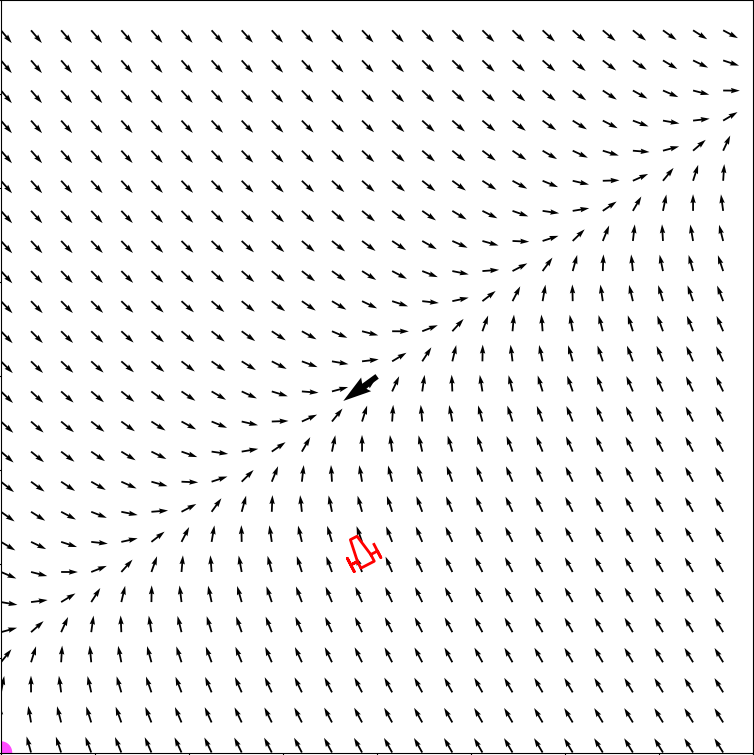
\includegraphics{imgs/ScreenshotCase1.png}}\resizebox{0.5\columnwidth}{!}{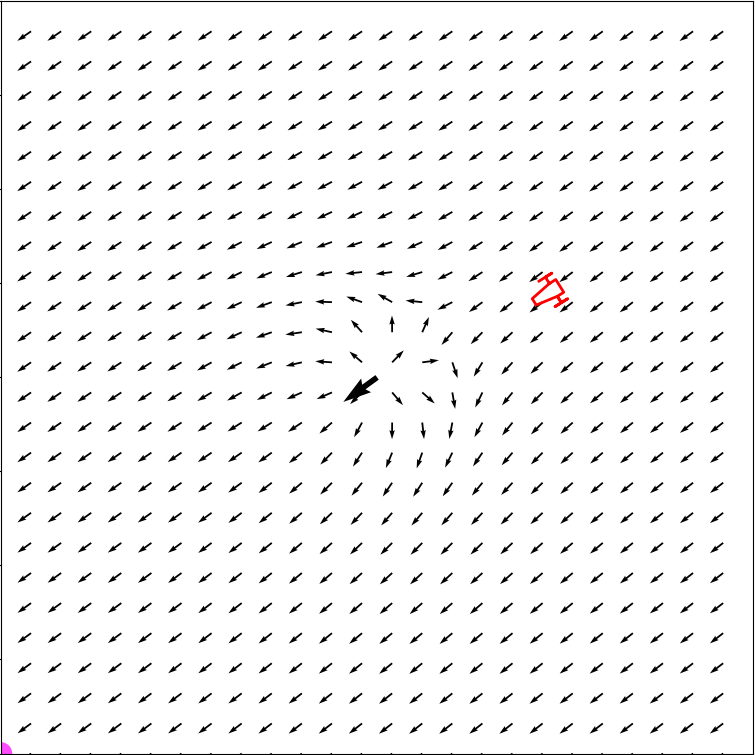
\includegraphics{imgs/ScreenshotCase2.png}}
  \caption{(a) Champ de vecteurs dans le premier cas. (b) Champ de vecteurs dans le second cas.}
\end{figure}

\section{Algorithme}

\chapter{Architecture logicielle}
\section{ROS}
Afin d'avoir un système efficace quand plusieurs parties doivent communiquer entre eux, il est essentiel
d'assurer une architecture logicielle claire et performante. Plusieurs choix s'offraient à nous à ce sujet,
étant équipés sur la plupart des éléments de ce système de carte NVIDIA Jetson, des cartes permettant moulte
options à ce sujet. En l'occurence, nous avons opté pour une architecture ROS, middleware très utilisé
dans notre domaine qui est la robotique.

\subsection{Présentation générale}
ROS (Robot Operating System) est un framework open source spécialement conçu pour le développement 
et la gestion de systèmes robotiques. Son architecture modulaire et distribuée offre aux développeurs
une base flexible et évolutive pour la création de systèmes robotiques sophistiqués.

Suivant un modèle de messagerie publish-subscribe, ROS facilite la communication transparente
entre les différentes composantes d'un système robotique, favorisant l'échange de données et de
commandes. Prenant en charge plusieurs langages de programmation, ce framework propose une
gamme complète d'outils et de bibliothèques qui simplifient le processus de développement.

L'infrastructure de communication dans ROS repose sur deux concepts fondamentaux: les nœuds
et les topics. Les nœuds sont des modules logiciels individuels, chacun réalisant une tâche spécifique
au sein du système robotique. Les nœuds, agissant comme les éléments fondamentaux d'une application ROS,
interagissent en échangeant des messages. D'autre part, les topics servent de canaux de communication
utilisés par les nœuds pour partager des messages au sein du framework ROS. Suivant
le modèle de communication publish-subscribe, les nœuds générant des données publient des messages sur
un topic spécifique, tandis que les nœuds intéressés par ces données souscrivent au topic correspondant
pour recevoir les messages.

\subsection{Limitations}

Contrairement à son successeur ROS2, ROS connait des limitations quand il s'agit de le mettre en place
sur un système composé de plusieurs parties. En effet, il est plus difficile de faire transiter les données
entre chaque machine sur ROS que ROS2. Alors que sur ROS2, être sur le même réseau suffit pour partager
les données entre les machines, ce n'est pas le cas sur ROS, ce qui complique la gestion de l'architecture
logicielle.

Malheureusement, les limitations logicielles ne nous permettaient pas de passer sur ROS2, étant équipés de
cartes NVIDIA Jetson flashées avec un équivalent de Ubuntu18, qui ne supporte pas ROS2.

De plus, tout est codé en \textit{python 2.7}, ce qui est également limitant dans nos capacités.

\section{Architecture du projet}

\begin{figure}[H]
    \centering
    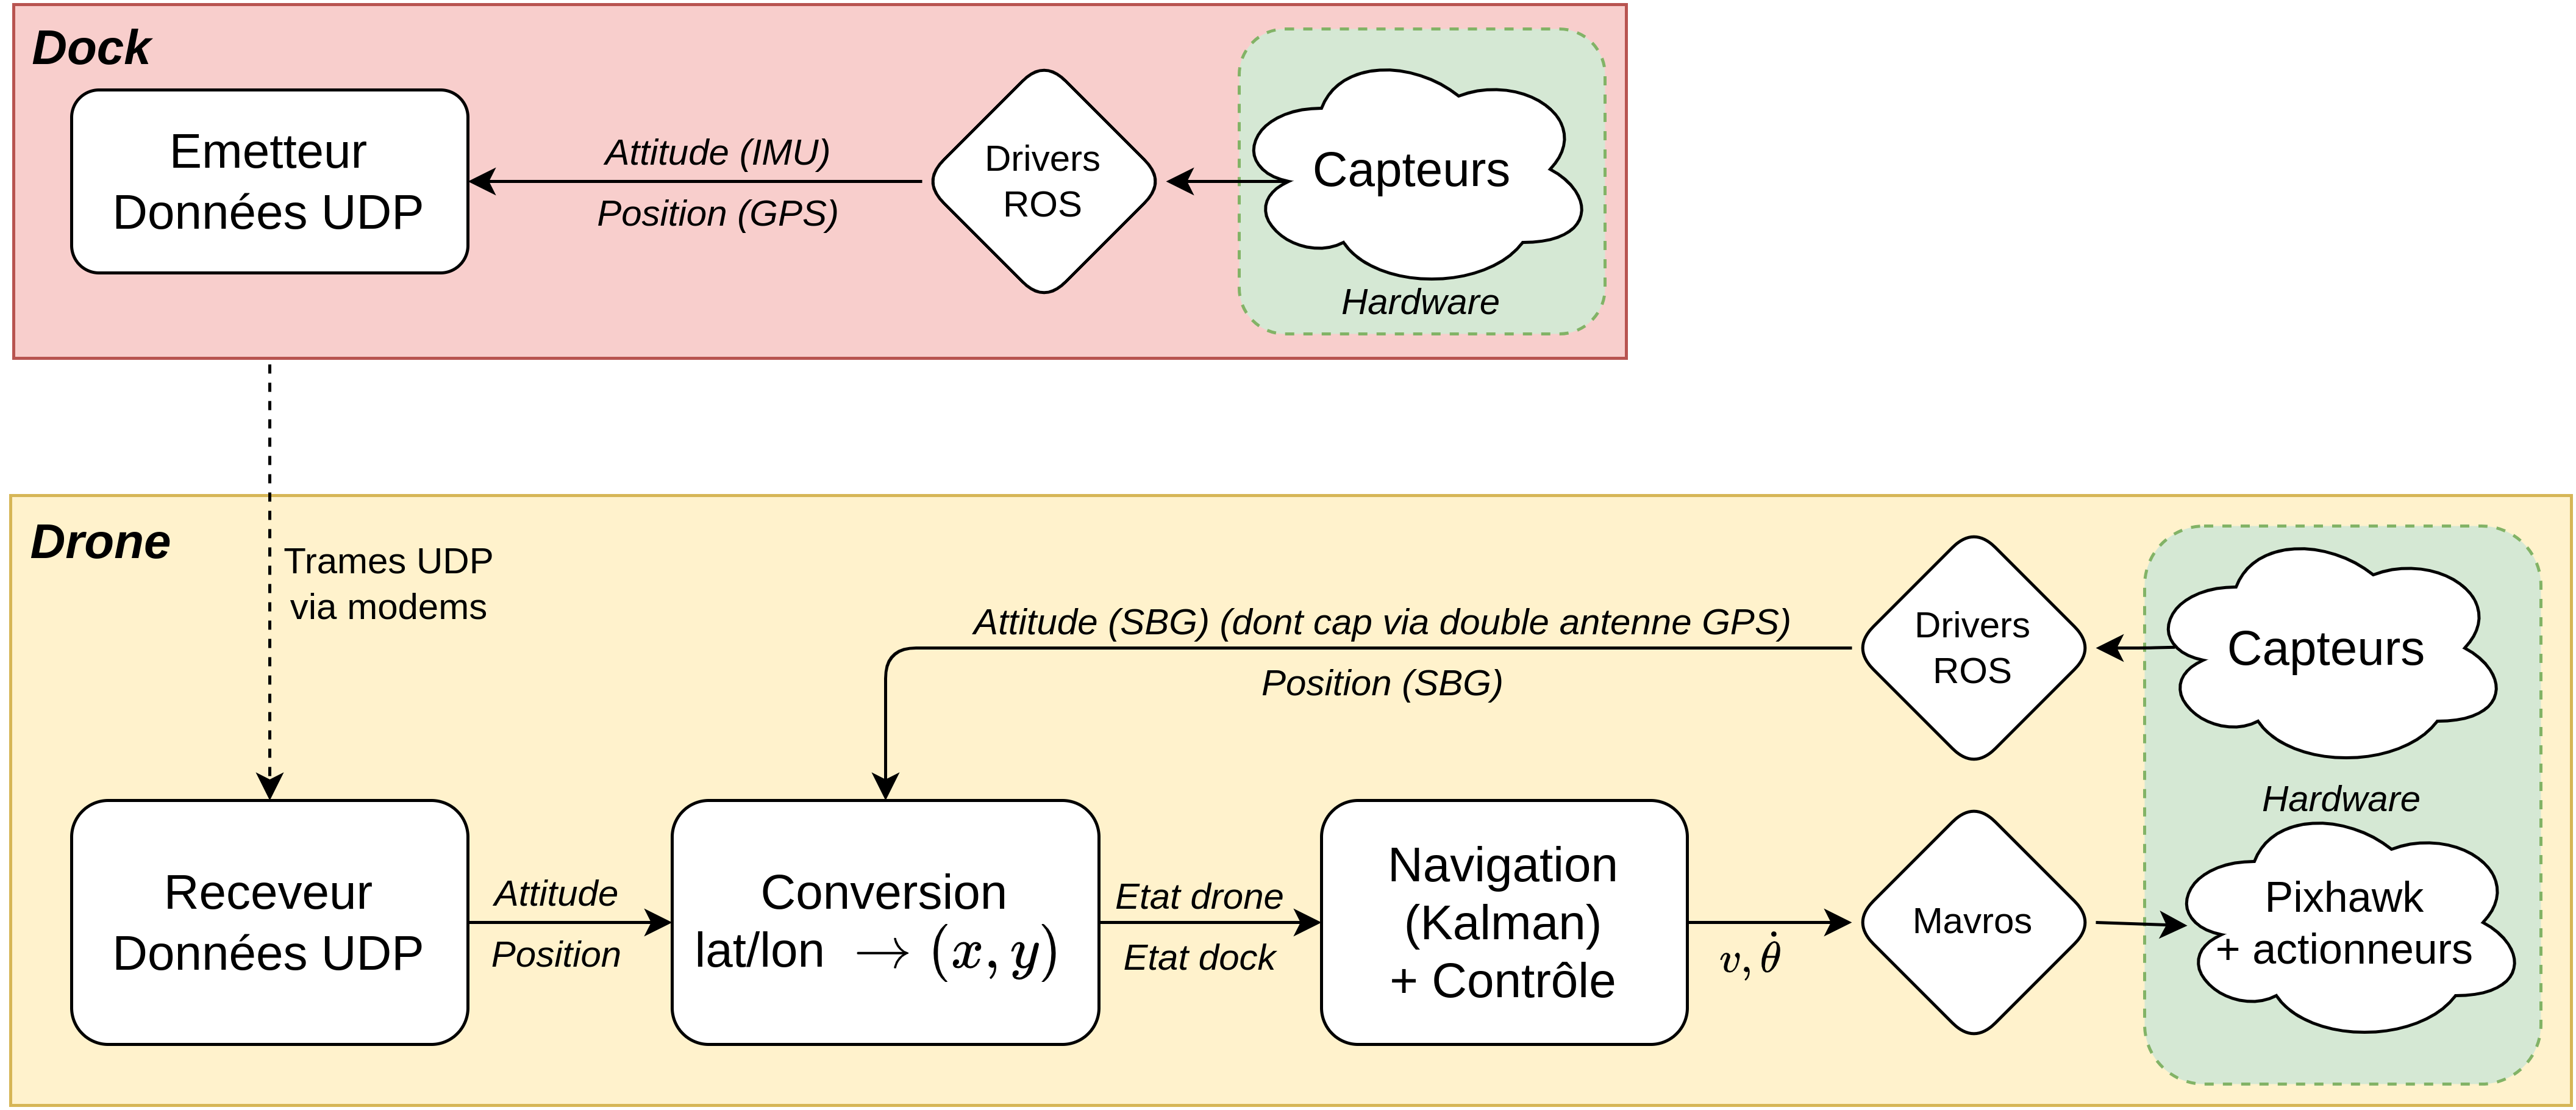
\includegraphics[width=0.95\textwidth]{imgs/schema_general.png}
    \caption{Architecture logicielle globale du système de docking}
    \label{fig:schema_general}
\end{figure}

\chapter{Essais à Guerlédan}

\section{Première semaine}

La première semaine d'expérimentations au lac de Guerlédan, du 9 au 13 octobre 2023, fut davantage une semaine de découverte du projet et permit une première approche à la résolution de notre problème. 
Durant cette semaine, nous avons rencontré nos encadrants et pris en main le matériel que nous avions à notre disposition, c'est-à-dire principalement les composants de ce qui sera plus tard notre dock,
que nous avons conçu durant cette semaine. Ainsi, à l'aide des composants décrits précédemment, nous avons été capable de créer la boite qui contient les capteurs nécessaires au bon fonctionnement du dock. 

D'autre part, nous travaillions en parallèle sur la mise en place de la correction RTK en configurant les différentes cartes et en prenant des mesures nécessaires au calcul de la correction. 

Enfin, une première version simplifiée de l'architecture logicielle a commencé à être implémentée. 


La principale problématique de cette semaine, qui est la même que celle rencontrée durant la période séparant cette semaine de la seconde, est l'impossibilité d'expérimenter directement sur l'AUV qui 
est le drone principal de notre sujet. En effet, l'avancée de notre projet ne nous permettait pas la sécurité de pouvoir tester nos algorithmes de manière sereine sur le drone et nous avons également 
rencontré quelques difficultés avec l'utilisation de l'interface MAVROS, qui fait le lien entre notre architecture ROS et MAVLink. Le principal problème résidait dans le fait qu'il semblait que MAVLink 
avait en mémoire des waypoints GPS que le drone tentait de rejoindre en priorité avant de prendre en compte nos commandes. Cela empêchait toute exploitation du drone en mode automatique, ce qui est nécessaire
au bon fonctionnement de nos algorithmes.

Heureusement ce problème avait tout le temps d'être réglé, étant donné que nous n'utiliserions pas le drone d'ici à la seconde semaine d'expérimentation à Guerlédan, en février 2024. De plus, nous avons 
décidé de concentrer nos efforts sur la mise en place et la conversion de nos algorithmes pour la mise en place sur le Rover qui nous sert de remplacement au drone et qui nous sert de moyen d'expérimentations à l'école. 


\section{Deuxième semaine}

La seconde semaine d'expérimentations, qui eut lieu du 5 au 9 février 2024, fut bien davantage une semaine d'expérimentation que la première. 
En effet, forts du travail effectué entre les deux semaines, nous avons été capables de mettre en oeuvre et tester nos algorithmes sur le drone principal.

La première étape préliminaire à cela fut de convertir nos codes, conçus pour fonctionner sur le rover, pour qu'ils puissent se mettre correctement en oeuvre sur le drone, qui, on le rappelle, n'est pas
équipé des mêmes capteurs et architecture logicielle des drivers. Il y a également des fonctionnalités supplémentaires sur le drone qui permettent plus de précision sur l'acquisition de l'état du drone, notamment 
l'obtention du \textit{True Heading}, sur lequel nous reviendrons plus tard, qui permet l'obtention du cap avec une plus grande fiabilité qu'en utilisant uniquement la centrale inertielle. 

Une des principales problématiques rencontrées durant la semaine réside dans la difficulté à bien calibrer les centrales inertielles. En effet, les centrales inertielles SBG nécessitent une étape de calibration
afin qu'elles compensent le champ magnétique disturbé pour calculer son attitude. Malgré de nombreux essais dans de nombreuses configurations, nous n'avons jamais réussi à bien configurer la centrale 
pour que la sortie de son filtre de Kalman concernant le cap ne diverge pas, surtout pour le dock. Si le dock reste trop longtemps immobile, sans perturbations, son cap se met à diverger rapidement.
Ce problème reste un point d'amélioration essentiel car il est une des raisons principales à l'absence d'expérimentations avec le vrai dock. 

Cependant, nous avons développé des alternatives permettant tout de même de mettre en oeuvre nos algorithmes en contournant le problème. Lorsque nous lancons le système, nous avons le choix entre
utiliser le vrai dock ou un dock simulé. Le dock simulé repose soit sur des logs d'essais précédents soit sur une position et orientation désirée précisées au lancement. 
En faisant cela, nous avons été capable de tester et prouver la robustesse de nos algorithmes, même sans présence du vrai dock.



\chapter{Conclusion}
\section{Résultats}

\section{Perspectives}
%//TODO mentionner : + de tests avec le vrai dock, approche avec d'autres capteurs (LIDAR, caméra)
Ce projet contient encore beaucoup d'aspects très intéressants à aborder. Un des premiers aspects à
approfondir est de faire plus de tests avec le dock.

De plus, il peut être intéressant d'enrichir la gamme de capteurs utilisés notamment pour l'étape du
docking en lui-même qui nécessite de la précision. Une perspective d'évolution serait d'utiliser par
exemple un LIDAR ou une caméra pour se docker bien plus précisément qu'avec uniquement le GPS et la
centrale inertielle.

Enfin, il pourrait également être envisageable d'intégrer des algorithmes d'évitement d'obstacles à
l'aide des nouveaux capteurs utilisés. L'ajout de cette fonctionnalité serait de plus compatible avec la
facon dont on procède, étant donné que l'on travaille avec des champs de vecteurs pour le contrôle, ce
qui est avantageux pour l'évitement d'obstacles.

\chapter{Annexes}
\section{Configuration des modules \textit{u-blox} avec \textit{U-Center}}
Pour configurer les modules GNSS \textit{u-blox}, il faut utiliser le logiciel \textit{U-Center} sous \textbf{Windows}. La carte doit être connectée par son port série \textbf{Power+GPS} à l'ordinateur.
\subsection{Configuration de la base}
Il faut d'abord se connecter au bon port \textit{COM} et choisir le bon \textit{baudrate}, normalement 9600.
Pour ouvrir la fenêtre de configuration, cliquer sur \textit{Configuration View}. Il faut ensuite renseiner les différents réglages suivants en appuyant bien sur \textbf{Send} à chaque modification : 
\begin{itemize}
    \item Onglet \textit{Msg} : cocher la case \textit{USB-On} et \textit{UART1-On} pour les messages suivants : 
    \begin{itemize}
        \item F5-05 RTCM3.3 1005
        \item F5-05 RTCM3.3 1077
        \item F5-05 RTCM3.3 1087
        \item F5-05 RTCM3.3 1127
        \item F5-05 RTCM3.3 1230
        \item 01-13 NAV-HPPOSECEF
        \item 01-02 NAV-POSLLH
        \item 02-15 RXM-RAWX
        \item 02-13 RXM-SFRBX
        \item F5-4A RTCM3.3 1074
        \item F5-4D RTCM3.3 1077
        \item F5-54 RTCM3.3 1084
        \item F5-57 RTCM3.3 1087
        \item F5-5E RTCM3.3 1094
        \item F5-61 RTCM3.3 1097
        \item F5-7C RTCM3.3 1124
        \item F5-7F RTCM3.3 1127
    \end{itemize}
    \item Onglet \textit{NMEA} : cocher \textit{High precision mode} pour le réglage \textit{CFG-NMEA(DATA2)}
    \item Onglet \textit{TIMEMODE3} : choisir le mode \textit{Survey-In} pour avoir un temps d'acquisition de la position et une précision minimale; ou le mode \textit{Fixed Mode} si la position précise est déjà connue. En mode d'acquisition longue, il faut prévoir plusieurs heures avant d'avoir une précision décimétrique.
    \item Onglet \textit{PRT} : 
    \begin{itemize}
        \item \textit{Target : 1-UART1, Protocol in : none, Protocol out : 0+1+5-UBX+NMEA+RTCM3, Baudrate : 115200, Databits : 0, Stopbits : 1, Parity : None, Bit Order : LSB First}
        \item \textit{Target : 3-USB, Protocol in : 0+1+5-UBX+NMEA+RTCM3, Protocol out : 0+1+5-UBX+NMEA+RTCM3}
    \end{itemize}
    \item Onglet \textit{CFG} : sélectionner toute la rubrique \textit{Devices}, s'assurer que \textit{Save current configuration} est coché, cliquer sur \textit{Send}.
\end{itemize}

\subsection{Configuration du dock}
Il faut d'abord se connecter au bon port \textit{COM} et choisir le bon \textit{baudrate}, normalement 9600.
Pour ouvrir la fenêtre de configuration, cliquer sur \textit{Configuration View}. Il faut ensuite renseiner les différents réglages suivants en appuyant bien sur \textbf{Send} à chaque modification : 
\begin{itemize}
    \item La configuration des messages du rover est optionnelle. Onglet \textit{Msg} : cocher la case \textit{USB-On} pour les messages : 
    \begin{itemize}
        \item \textit{F5-05 RTCM3.3 1005}
        \item \textit{F1-00 PUBX00}
        \item \textit{F1-03 PUBX03}
        \item \textit{F1-04 PUBX04}
    \end{itemize}
    Puis cocher aussi la case \textit{UART1-On} pour les messages :
    \begin{itemize}
        \item \textit{01-13 NAV-HPPOSECEF}
        \item \textit{01-02 NAV-POSLLH}
        \item \textit{F0-0A NMEA GxDTM}
        \item \textit{F0-00 NMEA GxGGA}
        \item \textit{F0-01 NMEA GxGLL}
        \item \textit{F0-02 NMEA GxGSA}
        \item \textit{F0-03 NMEA GxGSV}
    \end{itemize}
    \item Onglet \textit{NMEA} : cocher \textit{High precision mode} pour le réglage \textit{CFG-NMEA(DATA2)}.
    \item Onglet \textit{TIMEMODE3} : mode \textit{Disabled}.
    \item Onglet \textit{PRT} : 
    \begin{itemize}
        \item \textit{Target : 1-UART1, Protocol in : none, Protocol out : 0+1+5-UBX+NMEA+RTCM3}.
        \item \textit{Target : 3-USB, Protocol in : 0+1+5-UBX+NMEA+RTCM3, Protocol out : 0+1+5-UBX+NMEA+RTCM3}.
    \end{itemize}
    \item Onglet \textit{CFG} : sélectionner toute la rubrique \textit{Devices}, s'assurer que \textit{Save current configuration} est coché, cliquer sur \textit{Send}.
\end{itemize}

\subsection{Informations sur les LEDs}
\begin{center}
    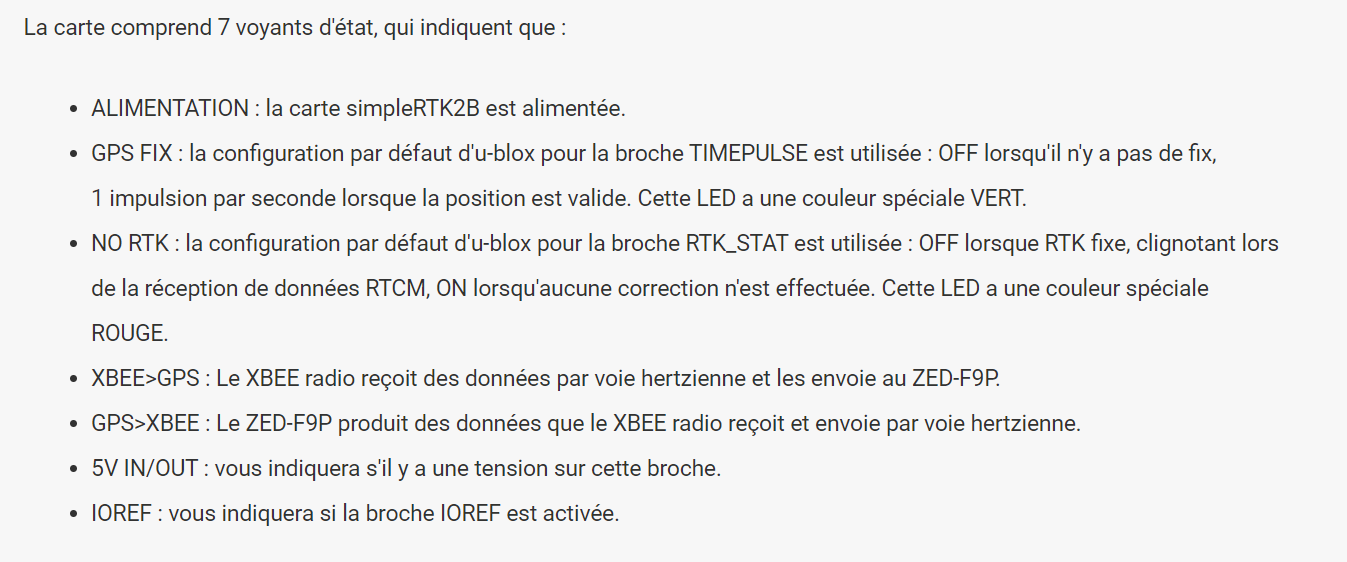
\includegraphics[width=0.8\textwidth]{imgs/led.png}
\end{center}

\section{Configuration des antennes \textit{XBEE S2C 2,4 GHz} avec \textit{XCTU}}
La configuration des antennes \textit{XBEE S2C 2,4 GHz} se fait avec le logiciel \textit{XCTU} sous \textbf{Windows}.
Il faut d'abord connecter le module par son port série \textit{Power+Xbee} à l'ordinateur.
En cas de problème avec le logiciel (impossibilité de détecter le module ou de lire ses paramètres), il faut court-circuiter les pins \textit{RESET N} et \textit{GND} du module pendant la configuration. Cela devrait résoudre le problème.
On clique sur \textit{Add a radio module} puis on choisit le bon port \textit{COM} et le bon \textit{baudrate}, normalement 115200. On clique ensuite sur \textit{Finish} pour valider.
Une fois que le module est ajouté, on clique sur les paramètres pour le configurer. 
Pour les deux antennes, on doit choisir le même \textit{PAN ID} et le même \textit{Channel} pour qu'elles puissent communiquer.
Il faut également faire correspondre les \textit{Destination Address High} et \textit{Destination Address Low} pour que les antennes puissent communiquer entre elles. L'idée est que le \textit{DH} de l'un soit le \textit{SH} de l'autre, et que le \textit{DL} de l'un soit le \textit{SL} de l'autre, et inversement.
On règle aussi \textit{RP} à 5. La seule chose qui va différer est le \textit{CE} qui doit être \textit{Enabled} pour la base et \textit{Disabled} pour le dock.


\bibliographystyle{plain}
\bibliography{mabiblio}

\end{document}
